\begin{figure}[htp]
    \centering

    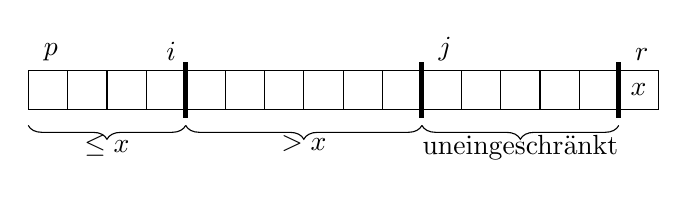
\begin{tikzpicture}
        % Squares
        \draw []    (0.0, 0.0) rectangle (0.5, 0.5) node[above left]{$p$};
        \draw []    (0.5, 0.0) rectangle (1.0, 0.5);
        \draw []    (1.0, 0.0) rectangle (1.5, 0.5);
        \draw []    (1.5, 0.0) rectangle (2.0, 0.5) node[above left]{$i$};

        \draw []    (2.0, 0.0) rectangle (2.5, 0.5);
        \draw []    (2.5, 0.0) rectangle (3.0, 0.5);
        \draw []    (3.0, 0.0) rectangle (3.5, 0.5);
        \draw []    (3.5, 0.0) rectangle (4.0, 0.5);
        \draw []    (4.0, 0.0) rectangle (4.5, 0.5);
        \draw []    (4.5, 0.0) rectangle (5.0, 0.5);

        \draw []    (5.0, 0.0) rectangle (5.5, 0.5) node[above left]{$j$};
        \draw []    (5.5, 0.0) rectangle (6.0, 0.5);
        \draw []    (6.0, 0.0) rectangle (6.5, 0.5);
        \draw []    (6.5, 0.0) rectangle (7.0, 0.5);
        \draw []    (7.0, 0.0) rectangle (7.5, 0.5);
        \draw []    (7.5, 0.0) rectangle (8.0, 0.5);
        \draw []    (7.5, 0.0) rectangle (8.0, 0.5) node[midway]{$x$} node[above left]{$r$};

        % Separators
        \draw[fill=black] (1.975, -0.1) rectangle (2.025, 0.6);
        \draw[fill=black] (4.975, -0.1) rectangle (5.025, 0.6);
        \draw[fill=black] (7.475, -0.1) rectangle (7.525, 0.6);
        
        % Braces
        \draw[decorate, decoration={brace, mirror, amplitude=5pt}]  (0.0, -0.2) -- node[below]{$\leq x$} (2.0, -0.2);
        \draw[decorate, decoration={brace, mirror, amplitude=5pt}]  (2.0, -0.2) -- node[below]{$> x$} (5.0, -0.2);
        \draw[decorate, decoration={brace, mirror, amplitude=5pt}] (5.0, -0.2) -- node[below]{uneingeschränkt} (7.5, -0.2);
    \end{tikzpicture}

    \caption{Die vier Regionen die von $\proc{Partition}$ auf einem Subarray $A[p \twodots r]$ behandelt werden. Die Werte in $A[p \twodots i]$ sind alle $\leq x$, die Werte in $A[i + 1 \twodots j - 1]$ sind alle $> x$, und $A[r] = x$. Das Subarray $A[j \twodots r - 1]$ kann jegliche Werte beinhalten. Die Abbildung und Beschreibung wurden aus \cite[173]{clrs2001}, Abbildung 7.2 übernommen.}
    \label{fig:quicks-partitioning}
\end{figure}